\chapter{Explorar o nosso ambiente}\label{ch:g6:exploring-our-environment}

Atravesse o pátio da escola ao meio-dia de julho e a face ensolarada
do muro estará quente debaixo da sua mão, o ar acima do asfalto vai
tremer, e a única coisa verde à vista será um matinho numa rachadura.
Passe para trás do muro sombreado: ar fresco, terra úmida, musgo,
tatuzinhos debaixo de uma pedra. Dois mundos, a três metros de
distância. Este ano começa explorando \omterm{def:g6:exploring-our-environment:components}{ambientes} do jeito que os
cientistas fazem --- medindo esses \omterm{def:g6:exploring-our-environment:components}{ambientes} e perguntando por que
cada \omterm{def:g6:exploring-our-environment:components}{ser vivo} mora exatamente onde mora.

\section{Do que um ambiente é feito}

\begin{definition}[Os componentes de um ambiente]\label{def:g6:exploring-our-environment:components}
Um \emph{ambiente}\index{ambiente} --- um pátio, um bosque, a margem
de uma lagoa --- contém três tipos de componentes:
\begin{enumerate}
  \item os \emph{seres vivos}\index{ser vivo}: os \omterm{def:g1:animals-around-us:animal}{animais}, as
        \omterm{def:g1:plants-around-us:plant}{plantas}, os cogumelos e a vida microscópica presentes;
  \item a \emph{matéria mineral}\index{matéria mineral}, que nunca
        esteve viva: rocha, pedra, a parte mineral do solo, a água,
        o ar;
  \item os \emph{vestígios e restos} de seres vivos: \omterm{def:g1:plants-around-us:parts}{folhas} secas,
        madeira caída, fezes, \omterm{def:g1:animals-around-us:covering}{penas}, \omterm{def:g1:animals-around-us:covering}{conchas} --- a caixa do ``já foi
        vivo'' da \cref{def:g1:living-or-not:nonliving}, agora um kit
        de pistas para quem explora.
\end{enumerate}
\end{definition}

\begin{example}[Inventário atrás do muro sombreado]\label{ex:g6:exploring-our-environment:inventory}
Dez minutos de inventário no canto fresco: \omterm{def:g6:exploring-our-environment:components}{seres vivos} --- musgo,
\omterm{prop:g4:plants-without-seeds:damp}{samambaias}, tatuzinhos, um caracol, uma centopeia, hera; mineral ---
a pedra do muro, terra úmida, uma poça; vestígios --- \omterm{def:g1:plants-around-us:parts}{folhas} secas,
uma \omterm{def:g1:animals-around-us:covering}{concha} de caracol, fezes de ave na cumeeira. Três listas, e o
canto está descrito como o sítio de um cientista.
\end{example}

\begin{omfigure}
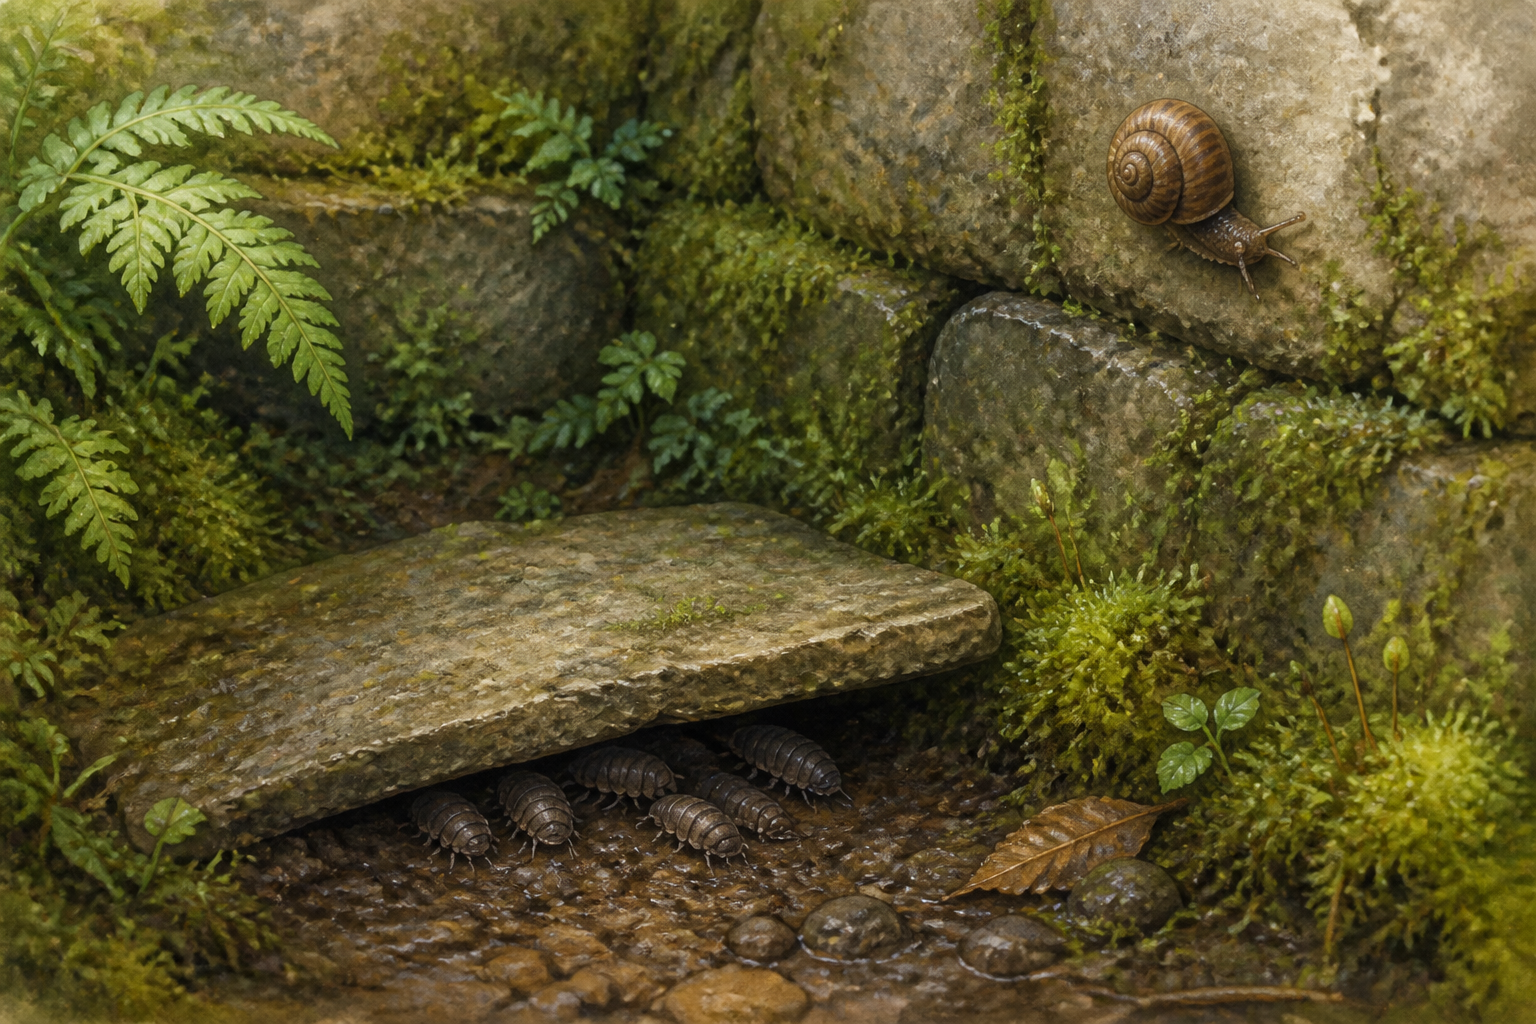
\includegraphics[width=0.62\linewidth]{images/book1/ai/g6-env-wallcorner.png}

{\small O canto fresco, no meio do inventário: musgo, \omterm{prop:g4:plants-without-seeds:damp}{samambaias}, um
caracol na pedra --- e, debaixo da laje levantada, o \omterm{def:g6:exploring-our-environment:microhabitat}{micro-hábitat}
dos tatuzinhos (recoloque a laje).}
\end{omfigure}

\begin{remark}[Os vestígios contam como dados]\label{rem:g6:exploring-our-environment:traces}
Quase todos os \omterm{def:g1:animals-around-us:animal}{animais} se escondem ou fogem, então quem explora
muitas vezes lê \emph{vestígios} no lugar deles: uma avelã roída dá
o nome do rato-do-mato, uma teia dá o nome da aranha dona dela,
pegadas na lama dão o nome da garça. Um inventário que só lista o
que ficou parado o bastante para ser visto perde metade dos
moradores.
\end{remark}

\section{Medir as condições}

\begin{definition}[Condições ambientais]\label{def:g6:exploring-our-environment:conditions}
As \emph{condições}\index{condições (ambientais)} de um \omterm{def:g6:exploring-our-environment:components}{ambiente} são
as características físicas mensuráveis dele:
\begin{itemize}
  \item a \emph{temperatura}\index{temperatura}, medida com um
        termômetro, em graus Celsius;
  \item a \emph{umidade}\index{umidade} --- o quanto o ar ou o solo
        estão úmidos;
  \item a \emph{luz}\index{luz (condição)} --- do sol pleno à sombra
        profunda.
\end{itemize}
As condições mudam de ponto para ponto --- muitas vezes de forma
brusca em poucos metros --- e ao longo do dia e do ano.
\end{definition}

\begin{example}[O pátio, medido]\label{ex:g6:exploring-our-environment:measured}
O levantamento do meio-dia de julho, com instrumentos: pé do muro
ensolarado --- \qty{38}{\degreeCelsius}, seco, sol pleno; canto
sombreado --- \qty{22}{\degreeCelsius}, terra úmida, sombra
profunda. Três metros de distância, dezesseis graus de diferença. Os
dois mundos do parágrafo de abertura agora são duas \emph{linhas de
uma tabela} --- e isso é um avanço, porque tabelas podem ser
comparadas.
\end{example}

\begin{proposition}[As condições decidem os moradores]\label{prop:g6:exploring-our-environment:decide}
Os \omterm{def:g6:exploring-our-environment:components}{seres vivos} de um ponto combinam com as \omterm{def:g6:exploring-our-environment:conditions}{condições} dele: cada
\omterm{def:g5:biodiversity:species}{espécie} prospera só dentro da faixa própria de \omterm{def:g6:exploring-our-environment:conditions}{temperatura}, \omterm{def:g6:exploring-our-environment:conditions}{umidade}
e \omterm{def:g6:exploring-our-environment:conditions}{luz}. O musgo e os tatuzinhos precisam de \omterm{def:g6:exploring-our-environment:conditions}{umidade} (o revestimento
do tatuzinho, ao contrário do de um inseto, deixa a água escapar ---
ele resseca fatalmente numa hora de sol); o matinho da rachadura
aguenta a seca e o brilho forte. Onde as \omterm{def:g6:exploring-our-environment:conditions}{condições} diferem, os
moradores diferem --- a regra por trás de todo \omterm{def:g2:where-animals-live:habitat}{hábitat} do
\cref{ch:g2:where-animals-live}.
\end{proposition}
\admitted

\begin{example}[O escolhedor de tatuzinhos]\label{ex:g6:exploring-our-environment:chooser}
A experiência clássica: uma caixa fechada, metade forrada com papel
úmido e metade com papel seco, e uma dúzia de tatuzinhos soltos ao
longo do meio. Em poucos minutos, quase todos estão do lado úmido.
Repita com uma metade sombreada contra uma metade iluminada: eles se
juntam na sombra. Ninguém os conduz --- cada \omterm{def:g1:animals-around-us:animal}{animal}, andando e
virando, acaba onde o corpo dele fica confortável. O mapa dos
tatuzinhos \emph{é} um mapa da \omterm{def:g6:exploring-our-environment:conditions}{umidade}.
\end{example}

\begin{method}[Levantar um sítio]\label{met:g6:exploring-our-environment:survey}
Para levantar um sítio pequeno como quem faz ciência de campo:
\begin{enumerate}
  \item escolha e marque uma área pequena --- um metro quadrado bem
        vasculhado conta mais do que um hectare olhado de relance;
  \item meça as \omterm{def:g6:exploring-our-environment:conditions}{condições}: \omterm{def:g6:exploring-our-environment:conditions}{temperatura}, \omterm{def:g6:exploring-our-environment:conditions}{umidade}, \omterm{def:g6:exploring-our-environment:conditions}{luz} --- mesmos
        instrumentos, mesmo jeito, em cada sítio (a regra de justiça
        do \cref{met:g4:what-plants-need:fairtest});
  \item faça o inventário dos três tipos de componentes --- \omterm{def:g6:exploring-our-environment:components}{seres
        vivos}, \omterm{def:g6:exploring-our-environment:components}{matéria mineral}, vestígios --- vasculhando direito:
        debaixo das pedras (recolocando as pedras:
        \cref{met:g2:caring-for-nature:rules}), nas frestas, embaixo
        das \omterm{def:g1:plants-around-us:parts}{folhas};
  \item registre tudo ali mesmo --- listas, esboços, contagens; a
        memória não é um instrumento de registro;
  \item compare os sítios: emparelhe cada diferença de moradores com
        uma diferença de \omterm{def:g6:exploring-our-environment:conditions}{condições}.
\end{enumerate}
\end{method}

\begin{remark}[Por que os registros ganham das lembranças]\label{rem:g6:exploring-our-environment:records}
De volta a lugar coberto, dois levantadores que confiaram na memória
vão discutir se os caracóis eram três ou cinco. O caderno resolve a
questão --- ou admite com honestidade que os caracóis não foram
contados. Os registros escritos, feitos no sítio, são o que
transforma um passeio em dados; todas as ciências deste livro
funcionam com eles.
\end{remark}

\section{Um ambiente, muitos micromundos}

\begin{definition}[Micro-hábitat]\label{def:g6:exploring-our-environment:microhabitat}
Dentro de um \omterm{def:g6:exploring-our-environment:components}{ambiente}, cada pontinho com \omterm{def:g6:exploring-our-environment:conditions}{condições} próprias e
moradores próprios --- a parte de baixo de uma pedra, uma rachadura
no muro, o pé sombreado da cerca viva --- é um
\emph{micro-hábitat}\index{micro-hábitat}. Os andares da floresta da
\cref{rem:g2:where-animals-live:layers} eram \omterm{def:g2:where-animals-live:habitat}{micro-hábitats}; o metro
quadrado de quem levanta um sítio em geral tem vários.
\end{definition}

\begin{example}[A pedra, por cima e por baixo]\label{ex:g6:exploring-our-environment:stone}
Uma pedra no canto fresco: em cima, líquen e uma mosca tomando sol
--- iluminado, seco, quente. Embaixo, tatuzinhos, uma centopeia,
\omterm{def:g1:plants-around-us:parts}{raízes} claras --- escuro, úmido, fresco. Dois \omterm{def:g6:exploring-our-environment:microhabitat}{micro-hábitats}
completos separados por cinco centímetros de rocha, cada um habitado
exatamente pelos \omterm{def:g6:exploring-our-environment:components}{seres vivos} cujas faixas combinam com as \omterm{def:g6:exploring-our-environment:conditions}{condições}
dele.
\end{example}

\section{Exercícios}

\begin{exercise}[$\star$]\label{exo:g6:exploring-our-environment:1}
Diga os três tipos de componentes de um \omterm{def:g6:exploring-our-environment:components}{ambiente}, com dois exemplos
de cada um tirados do inventário do canto sombreado.
\end{exercise}

\begin{exercise}[$\star$]\label{exo:g6:exploring-our-environment:2}
Que \omterm{def:g6:exploring-our-environment:conditions}{condições} quem faz ciência de campo mede num sítio, e com o quê
(onde um instrumento foi citado)?
\end{exercise}

\begin{exercise}[$\star$]\label{exo:g6:exploring-our-environment:3}
Separe nos três tipos de componentes: uma samambaia, uma \omterm{def:g1:animals-around-us:covering}{concha} de
caracol, uma poça, fezes de ave, uma centopeia, a pedra do muro.
\end{exercise}

\begin{exercise}[$\star$]\label{exo:g6:exploring-our-environment:4}
A partir do \cref{ex:g6:exploring-our-environment:measured}: quais
são as diferenças de \omterm{def:g6:exploring-our-environment:conditions}{temperatura} e de \omterm{def:g6:exploring-our-environment:conditions}{luz} entre os dois pontos? Que
moradores combinam com cada um?
\end{exercise}

\begin{exercise}[$\star$]\label{exo:g6:exploring-our-environment:5}
Por que o tatuzinho morre numa hora de sol, e o que isso explica
sobre onde os tatuzinhos são encontrados?
\end{exercise}

\begin{exercise}[$\star$]\label{exo:g6:exploring-our-environment:6}
Diga três vestígios e o \omterm{def:g1:animals-around-us:animal}{animal} que cada um deles nomeia, como na
\cref{rem:g6:exploring-our-environment:traces}.
\end{exercise}

\begin{exercise}[$\star\star$]\label{exo:g6:exploring-our-environment:7}
Descreva a experiência do escolhedor de tatuzinhos: montagem,
resultado e o que ela mostra --- sem ninguém conduzir os \omterm{def:g1:animals-around-us:animal}{animais}.
\end{exercise}

\begin{exercise}[$\star\star$]\label{exo:g6:exploring-our-environment:8}
Por que as \omterm{def:g6:exploring-our-environment:conditions}{condições} precisam ser medidas do mesmo jeito em cada
sítio? De que método anterior esta é a versão de campo?
\end{exercise}

\begin{exercise}[$\star\star$]\label{exo:g6:exploring-our-environment:9}
Dê os dois \omterm{def:g6:exploring-our-environment:microhabitat}{micro-hábitats} da pedra do
\cref{ex:g6:exploring-our-environment:stone}, com as \omterm{def:g6:exploring-our-environment:conditions}{condições} deles
e um morador de cada.
\end{exercise}

\begin{exercise}[$\star\star$]\label{exo:g6:exploring-our-environment:10}
Um levantamento registra ``uns bichos, estava meio quente''. Reescreva
as instruções de quem levantou usando o
\cref{met:g6:exploring-our-environment:survey} --- o que deveria ter
sido feito em cada passo?
\end{exercise}

\begin{exercise}[$\star\star$]\label{exo:g6:exploring-our-environment:11}
A hera sobe pelo muro sombreado, mas não pelo ensolarado. Proponha
uma explicação no formato da
\cref{prop:g6:exploring-our-environment:decide} e uma observação ou
medida que testaria essa explicação.
\end{exercise}

\begin{exercise}[$\star\star\star$]\label{exo:g6:exploring-our-environment:12}
Na caixa dos tatuzinhos, um aluno faz uma objeção: ``talvez eles
tenham só se juntado perto da parede, e por acaso o lado úmido
tivesse mais parede''. Planeje uma versão melhorada da experiência
que responda à objeção. (Pense em teste justo.)
\end{exercise}

\section{Problema: As duas valas}

\begin{problem}[{Problema de fim de semana --- o clube de
naturalistas levanta duas valas de beira de estrada e encontra dois
mundos diferentes}]\label{pb:g6:exploring-our-environment:1}
O clube de naturalistas levanta duas valas ao longo da mesma
estradinha, a $50$ metros uma da outra. A vala N corre pelo lado
sombreado de uma cerca viva alta; a vala S fica no aberto, exposta
ao sol o dia inteiro. O clube trabalha conforme as regras: mesmos
instrumentos, mesmo metro quadrado por sítio, mesmo tempo de busca.

\medskip\noindent\textbf{Parte I --- As medidas.}
\begin{enumerate}
  \item Os termômetros marcam \qty{19}{\degreeCelsius} na vala N e
        \qty{31}{\degreeCelsius} na vala S na mesma hora. Que
        característica dos sítios explica melhor essa diferença?
  \item A terra da vala N gruda nos dedos; a da vala S se esfarela
        em pó. Traduza as duas observações para o vocabulário da
        \cref{def:g6:exploring-our-environment:conditions}.
  \item O clube mede ao meio-dia. Dê um motivo pelo qual a
        comparação seria menos justa se a vala N fosse medida ao
        meio-dia e a vala S às 18 horas.
  \item Por que o clube usa a \emph{mesma} moldura de um metro
        quadrado e o mesmo tempo de busca nos dois sítios?
\end{enumerate}

\medskip\noindent\textbf{Parte II --- Os inventários.}
\begin{enumerate}[resume]
  \item A lista da vala N: musgo, \omterm{prop:g4:plants-without-seeds:damp}{samambaias}, tatuzinhos, caracóis,
        um sapo. A lista da vala S: capins secos, um matagal grande
        de \omterm{def:g1:plants-around-us:parts}{folhas} enceradas, formigas, um lagarto tomando sol,
        gafanhotos. Separe os \omterm{def:g1:my-body:parts}{membros} de cada lista nos três tipos de
        componentes --- e repare no que falta nas listas (confira a
        \cref{def:g6:exploring-our-environment:components}).
  \item Para cada um dos tatuzinhos, do sapo e do lagarto, diga as
        \omterm{def:g6:exploring-our-environment:conditions}{condições} de qual vala combinam com as necessidades dele, e
        por quê (use a
        \cref{prop:g6:exploring-our-environment:decide} e o que você
        sabe de cada \omterm{def:g1:animals-around-us:animal}{animal}).
  \item Na vala S o clube encontra uma \omterm{def:g1:animals-around-us:covering}{concha} de caracol, mas nenhum
        caracol, e pergunta se há caracóis morando ali. Que duas
        possibilidades honestas um vestígio assim deixa em aberto?
  \item Debaixo de uma pedra chata na vala N: oito tatuzinhos, uma
        centopeia, \omterm{def:g1:plants-around-us:parts}{raízes} brancas. Diga as \omterm{def:g6:exploring-our-environment:conditions}{condições} desse
        \omterm{def:g6:exploring-our-environment:microhabitat}{micro-hábitat} e enuncie a regra que pôs aqueles moradores ali.
\end{enumerate}

\medskip\noindent\textbf{Parte III --- A explicação.}
\begin{enumerate}[resume]
  \item Emparelhe cada diferença de moradores com uma diferença de
        \omterm{def:g6:exploring-our-environment:conditions}{condições}: complete ``a N tem musgo e sapos porque \dots; a S
        tem lagartos e matagais de \omterm{def:g1:plants-around-us:parts}{folhas} enceradas porque \dots''.
  \item A cerca viva está marcada para ser arrancada. Preveja as
        \omterm{def:g6:exploring-our-environment:conditions}{condições} da vala N dois verões depois --- e os moradores
        dela, usando o emparelhamento da questão 9.
  \item Um \omterm{def:g1:my-body:parts}{membro} propõe conferir a previsão direito: levantar as
        duas valas de novo depois que a cerca viva sumir. Por que os
        \emph{mesmos} sítios, instrumentos e estação do ano precisam
        ser usados para o novo levantamento valer?
  \item O relatório do clube termina assim: ``os moradores mapeiam as
        \omterm{def:g6:exploring-our-environment:conditions}{condições}''. Explique a frase com o escolhedor de tatuzinhos
        (\cref{ex:g6:exploring-our-environment:chooser}) e diga por
        que não é preciso conduzir ninguém para um mapa desses se
        desenhar sozinho.
\end{enumerate}
\end{problem}
